\documentclass[runningheads]{llncs}

\usepackage[T1]{fontenc}
\usepackage{graphicx}
\usepackage{booktabs}
\usepackage{amsmath}
\usepackage{xcolor}
\usepackage{array}
\usepackage{microtype}
\usepackage{tikz}
\usetikzlibrary{positioning,arrows.meta,fit,backgrounds}
\usepackage[hidelinks]{hyperref}
\setlength{\emergencystretch}{1.5em}
\renewcommand{\topfraction}{0.9}
\renewcommand{\textfraction}{0.1}
\renewcommand{\floatpagefraction}{0.8}
\setcounter{topnumber}{3}

\newcolumntype{L}[1]{>{\raggedright\arraybackslash}p{#1}}

\begin{document}

\title{Traceable by Construction: Evidence-Grounded LLM Analysis of Thai Cybercrime Cases}
\titlerunning{Traceable by Construction}

\author{Thattapon Surasak\inst{1} \and Kritsakorn Kahmwiset\inst{1}}
\authorrunning{T. Surasak and K. Kahmwiset}
\institute{Department of Computer and Information Science, Faculty of Applied Science,\\
King Mongkut's University of Technology North Bangkok, Bangkok, Thailand\\
\email{thattapon.s@sci.kmutnb.ac.th}, \email{s6604062630021@kmutnb.ac.th}}

\maketitle

\begin{abstract}
Large language models (LLMs) can summarise cybercrime complaints that span several documents, but an
investigator cannot act on a summary without knowing which sentence of which document supports
each statement, and citations written by the model are as fragile as the rest of its output. We
present a case-analysis system that makes traceability a property of the system rather than a
request in the prompt. Case documents are partitioned into Source units with exact offsets and stable
identifiers; a Reader LLM may only \emph{select} identifiers when writing a Claim, and the
system reproduces the quoted text from storage. A frozen Claim/Source check (multilingual sentence selection,
NLI and a logistic decision boundary) then labels each Claim, and every summary sentence must end
with the identifiers of the Claims it rests on. On WiCE the check improves Macro-F1 over
thresholded NLI by 0.033 (95\% CI 0.013--0.053). On AttributionBench, machine translation into
Thai raises its false acceptance by 17.4 points in-domain and 4.4 out-of-domain. In a paired
replay, using the check as a hard gate cut the share of unsupported benchmark Claims cited in
summaries from 100\% to 22.2\% ($p=0.016$) but withheld 31\% of supported Claims, so the deployed
system shows the verdict as a warning instead. Accuracy on native Thai case files remains
unmeasured.

\keywords{Evidence traceability \and Large language models \and Claim verification \and
Natural language inference \and Cybercrime investigation \and Thai language}
\end{abstract}

%======================================================================
\section{Introduction}
%======================================================================

Cybercrime complaints rarely arrive as one clean narrative. A typical case holds a victim's
account, screenshots of chats, bank transfer slips and scanned police forms, much of it in Thai
and much of it recovered by optical character recognition (OCR). LLMs can condense such a case
into a readable summary, but they also produce fluent statements that no source supports
\cite{ji2023hallucination}. In an investigation, an unsupported amount, date or name is not a
stylistic flaw: it can send an officer after the wrong account, or put a wrong figure into a
request to freeze funds.

The common remedy is to make the model cite: attributed-generation methods train or
prompt models to attach citations or quoted spans to each sentence
\cite{gao2023alce,slobodkin2024afg}. Domain workflows go further and label every output unit
with an explicit evidence identifier \cite{yang2026traceable}. In all of these, however, the
pointer is still text written by the model, so its existence and accuracy must be checked
afterwards, often by people. A wrong citation looks exactly like a correct one to a busy reader.

Thai adds two difficulties. Sentence boundaries are not marked by punctuation, so even deciding
what to quote requires a segmenter \cite{phatthiyaphaibun2023pythainlp}; and most claim
verification resources and checkpoints are English. The multilingual NLI checkpoint we use, for
example, was deliberately trained without Thai NLI data \cite{laurer2022mdeberta}. Any semantic
check a Thai system relies on is therefore a cross-lingual transfer whose behaviour has to be
measured, not assumed.

We take a different position: \emph{the model chooses evidence; the system owns it}.
The model never writes a quotation, an offset or a page number. It may only select identifiers
that the system issued for spans it can reproduce byte for byte, and everything the user sees as
evidence is regenerated from storage. Our contributions are:
\begin{enumerate}
\item An analysis architecture in which a claims-only Reader selects system-issued Source-unit
identifiers, deterministic binding resolves them to original spans with document and page locators, and a
separate Judgement stage writes a summary over Claims alone, ending each sentence with Claim
identifiers (Sects.~\ref{sec:problem}--\ref{sec:system}).
\item A frozen Claim/Source check, B1-LR, built from off-the-shelf multilingual models and a
three-weight logistic boundary, with its design decisions and an English checkpoint comparison,
evaluated on WiCE, on AttributionBench, and on a Thai machine translation of AttributionBench
(Sect.~\ref{sec:eval}).
\item A paired downstream replay that quantifies the coverage cost of using such a check as a
filter, and the resulting design decision to deploy it as a warning label
(Sects.~\ref{sec:replay} and~\ref{sec:discussion}).
\end{enumerate}
The setting is a public-safety service where trustworthiness has to be inspectable: every
statement an officer reads should lead back to a document, a page and a character range.

%======================================================================
\section{Related Work}
%======================================================================

Two lines of work meet in this paper: traceability, which asks whether an output can be followed
back to what produced it, and attribute-first generation, which makes evidence selection an explicit
step before writing. We also draw on claim verification for the semantic check.

\subsection{Traceability and Provenance}

Traceability has a long history outside NLP. In requirements engineering it is the ability to
follow the life of a requirement both forwards and backwards; Gotel and Finkelstein argued that many
problems stem from missing information about where an artifact came from and how it was produced
\cite{gotel1994traceability}. Database research distinguishes \emph{why}-provenance, the
source records that justify an output, from \emph{where}-provenance, the exact location a value was
copied from \cite{buneman2001provenance}; W3C PROV standardises the entities, activities and agents
needed to record such histories \cite{lebo2013provo}. Our design maps directly onto this vocabulary:
a citation is where-provenance (a source and a character range), the Claim identifiers on a summary
sentence are why-provenance, and both are recorded when the output is produced rather than
reconstructed afterwards.

For LLM output, the need is well documented. An audit of four generative search engines found that
only 51.5\% of generated sentences were fully supported by their citations and only 74.5\% of
citations supported the sentence they were attached to \cite{liu2023verifiability}. Domain
systems respond with explicit evidence records. Yang et al.\ register exhibition evidence under
stable identifiers and label each generated unit as grounded or creative, auditing the links
manually \cite{yang2026traceable}; Dehing et al.\ carry message trace identifiers into structured
forensic reports \cite{dehing2026forensics}; Worledge et al.\ locate every quote on its court-file
page \cite{worledge2026default}. In each case the identifier or quote is written by the model and
checked afterwards; in ours it is issued and resolved by the system.

\subsection{Attribute First, then Generate}

Attributed question answering frames attribution as a task in its own right
\cite{bohnet2022attributedqa}, and attribution is commonly judged by whether a statement is
supported by an identified source \cite{rashkin2023ais}. Two families of methods followed.
\emph{Post-hoc} methods generate first and attach or repair evidence later: RARR searches for
evidence for an existing output and revises unsupported content \cite{gao2023rarr}, and ALCE
benchmarks models that cite retrieved passages while writing \cite{gao2023alce}. \emph{Attribute-first}
methods invert the order. Slobodkin et al.\ select concise source spans, cluster them into a
sentence-level plan, and only then generate, discarding selected spans that cannot be found in the
source \cite{slobodkin2024afg}; this shortened human verification time in both of their tasks,
while human-judged attribution rose in one task and fell in the other.

Later work refines the selected unit and what is done with it. FRONT trains models to extract
fine-grained quotes before writing grounded citations \cite{huang2024front}; GenerationPrograms
expresses the answer as an executable program of operations over source sentences, so that each
output sentence carries its derivation \cite{wan2025generationprograms}; Worledge et al.\ show
that moving from quotation toward abstraction makes answers more fluent and useful but harder and
slower to verify \cite{worledge2024spectrum}; CiteLab provides tooling to compare citation workflows,
attribute-first among them \cite{shen2025citelab}; and QA-based propositions can localise exactly
which part of an attributed sentence is inconsistent with its source \cite{cattan2026localizing}.
In domains, Worledge et al.\ apply attribute-first generation to legal default-judgment review with
a randomised study of law students \cite{worledge2026default}, MedGraphRAG uses it as a baseline for
evidence-based medical answers \cite{wu2025medgraphrag}, FinRAGBench-V moves the evidence unit to
page images and bounding boxes \cite{zhao2025finragbenchv}, and evidence-based QA specialists are
trained on data filtered for source quality and attributability \cite{schimanski2024specialists}.

We keep the attribute-first order but change what is selected. The Reader selects opaque identifiers
issued by the system instead of copying spans, so the existence check that attribute-first methods
perform by string matching becomes an exact lookup, and a quotation can never drift from its source.

\subsection{Claim Verification}

A third line checks generated text against evidence. FActScore checks atomic facts
\cite{min2023factscore}, SummaC applies sentence-level NLI to summaries \cite{laban2022summac},
MiniCheck trains small grounding checkers \cite{tang2024minicheck}, and AttrScore judges attribution
with LLMs and fine-tuned models \cite{yue2023attrscore}; WiCE \cite{kamoi2023wice} and
AttributionBench \cite{li2024attributionbench} supply labelled claim/evidence pairs. For Thai, XNLI
provides professionally translated NLI test data \cite{conneau2018xnli}, and PyThaiNLP provides
sentence segmentation \cite{phatthiyaphaibun2023pythainlp}. We do not propose a new checker: we
assemble a cheap, frozen one from multilingual components \cite{reimers2020multilingual} and measure
what it does at one point in the pipeline. Table~\ref{tab:related} summarises the positioning.

\begin{table}[t]
\centering
\caption{Positioning by evidence pointer. ``Checked'' describes how the system or study tests
the pointer, as reported by each paper.}
\label{tab:related}
\footnotesize
\setlength{\tabcolsep}{3pt}
\begin{tabular}{L{1.9cm}L{1.7cm}L{2.4cm}L{2.5cm}L{2.5cm}}
\toprule
Work & Domain & Evidence pointer & Checked & Evaluation \\
\midrule
ALCE \cite{gao2023alce} & Open QA & Model writes passage citations & NLI-based metric at evaluation & Automatic benchmark \\
AfG \cite{slobodkin2024afg} & Summaries, long-form QA & Model selects source spans & Span string match & Human attribution, time \\
Worledge et al.\ \cite{worledge2026default} & Court review & Model selects quotes & Fuzzy match, replaced by source text & Randomised user study \\
Dehing et al.\ \cite{dehing2026forensics} & Chat forensics & Trace identifiers & Per-field evaluation & Entity, role, timeline \\
Yang et al.\ \cite{yang2026traceable} & Exhibit design & Model writes evidence IDs & Manual unit audit & Two experts \\
\textbf{Ours} & Thai cyber-crime cases & Model selects system-issued unit IDs & Deterministic resolution; B1-LR per Claim at runtime & WiCE, AttributionBench EN/MT-TH, replay \\
\bottomrule
\end{tabular}
\end{table}

%======================================================================
\section{Problem Setting and Requirements}\label{sec:problem}
%======================================================================

A \emph{case} $K$ owns a set of sources $S_1,\dots,S_m$. A source is a string: a narrative typed by
the user or the text extracted from an uploaded document, with page locators where they exist. An
analysis of $K$ produces a set of \emph{Claims} $c_1,\dots,c_n$, each a short proposition with a
type, an epistemic status and two citation lists (supporting and contradicting), and a summary
$\Sigma = (\sigma_1,\dots,\sigma_k)$ whose sentences each reference a non-empty subset of Claims.
A \emph{citation} is a triple $(S_i, a, b)$ denoting the substring $S_i[a{:}b]$.

From the task itself (an investigator must be able to justify each statement in a case file) and
from earlier versions of our system in which the model wrote its own quotations, which then had to be
matched back to the sources approximately, we derived five requirements:
\textbf{R1 Verbatim evidence}: every quotation shown is a substring of a stored source, reproduced
by the system, never by a model. \textbf{R2 Fail visibly}: an unresolvable pointer is shown as
invalid, not dropped or repaired. \textbf{R3 Revision safety}: a pointer issued for one version of a
document never binds to another. \textbf{R4 Sentence-level provenance}: every summary sentence names
the Claims it rests on, and only Claims the analysis produced. \textbf{R5 Bounded cost}: expensive
stages run only when the case is complete enough, and any semantic check is cheap enough for every
Claim.
R1--R4 are structural and can be enforced by construction; R5 shapes the pipeline. Whether a
Claim is \emph{true}, or even entailed by its citations, is a separate question that no structural
rule answers, which is what the Claim/Source check in Sect.~\ref{sec:check} addresses, imperfectly.

%======================================================================
\section{System Design}\label{sec:system}
%======================================================================

\begin{figure}[t]
\centering
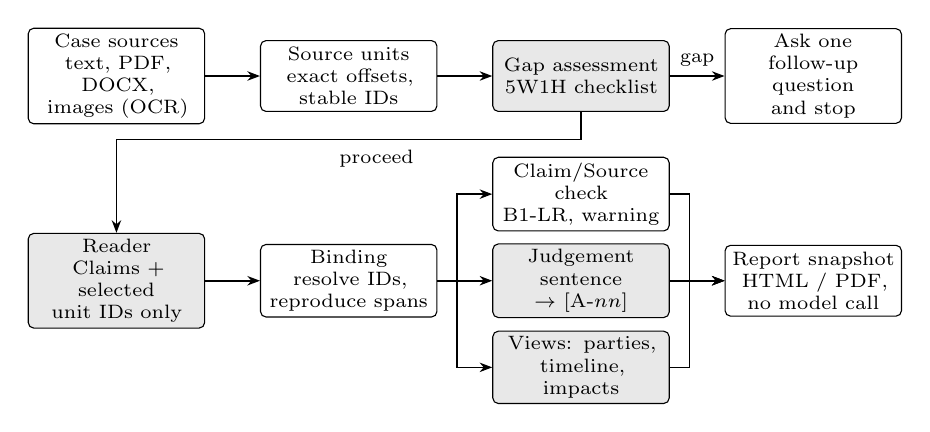
\begin{tikzpicture}[
  font=\scriptsize,
  box/.style={draw, rounded corners=2pt, align=center, minimum height=9mm, inner sep=2pt, text width=21mm},
  llm/.style={box, fill=gray!18},
  det/.style={box, fill=white},
  arr/.style={-{Stealth[length=1.6mm]}, semithick}]
% row 1: intake and preflight
\node[det] (src)    at (0,0)     {Case sources\\ text, PDF, DOCX,\\ images (OCR)};
\node[det] (units)  at (2.95,0)  {Source units\\ exact offsets,\\ stable IDs};
\node[llm] (assess) at (5.9,0)   {Gap assessment\\ 5W1H checklist};
\node[det] (ask)    at (8.85,0)  {Ask one\\ follow-up question\\ and stop};
% row 2: analysis, fan-out after binding, fan-in to the report
\node[llm] (reader) at (0,-2.6)  {Reader\\ Claims + selected\\ unit IDs only};
\node[det] (bind)   at (2.95,-2.6) {Binding\\ resolve IDs,\\ reproduce spans};
\node[det] (check)  at (5.9,-1.5)  {Claim/Source check\\ B1-LR, warning};
\node[llm] (judge)  at (5.9,-2.6)  {Judgement\\ sentence $\to$ [A-$nn$]};
\node[llm] (views)  at (5.9,-3.7)  {Views: parties,\\ timeline, impacts};
\node[det] (report) at (8.85,-2.6) {Report snapshot\\ HTML / PDF,\\ no model call};
\draw[arr] (src) -- (units);
\draw[arr] (units) -- (assess);
\draw[arr] (assess) -- node[above]{gap} (ask);
\draw[arr] (assess.south) -- ++(0,-0.35) -| node[pos=0.22, below]{proceed} (reader.north);
\draw[arr] (reader) -- (bind);
\draw[arr] (bind.east) -- ++(0.25,0) |- (check.west);
\draw[arr] (bind.east) -- (judge.west);
\draw[arr] (bind.east) -- ++(0.25,0) |- (views.west);
\draw[arr] (check.east) -- ++(0.25,0) |- (report.west);
\draw[arr] (judge.east) -- (report.west);
\draw[arr] (views.east) -- ++(0.25,0) |- (report.west);
\end{tikzpicture}
\caption{Analysis flow. Shaded boxes call an LLM; white boxes are deterministic or
use frozen local models. The Reader can only select identifiers that the system issued, and the
Claim/Source check, Judgement and Views run concurrently after binding.}
\label{fig:pipeline}
\end{figure}

Figure~\ref{fig:pipeline} summarises the flow. Every PDF page is rendered and read by OCR rather than taken from the PDF's text layer,
and page locators are kept. The system writes in Thai whenever any source contains
a Thai character, and a chat question is answered in its own language.

\paragraph{Source units (R1, R3).}
At analysis time each source is partitioned into units that reuse sentence boundaries (Thai
sentence segmentation with PyThaiNLP's CRF model \cite{phatthiyaphaibun2023pythainlp}; table rows
become their own units) and preserve all separators. Every unit satisfies
$\mathit{text} = \mathit{source}[\mathit{start}{:}\mathit{end}]$, and the ordered units
reconstruct the source exactly. A canonical identifier has the form
\texttt{source\_id:U001-}$h$, where $h$ is 16 hexadecimal characters derived from the
segmentation version and the full source text, so an identifier issued for one revision of a
document cannot silently bind to another. Units are computed on demand, not stored.

\paragraph{Gap assessment before expensive work (R5).}
A cheap first LLM call checks the case against a fixed 5W1H checklist (who was affected, who was
responsible, what, when, where, why, how and how much). A deterministic policy then either asks the
user and stops, or proceeds. Rounds and questions are bounded, and answers are stored with their own
identifiers (\texttt{QA-01}) rather than as case sources.

\paragraph{Claims-only Reading.}
The Reader receives all sources with compact local identifiers (\texttt{U001}, \dots) together with
document and extraction-quality metadata, and returns a strict JSON object with a version and a list
of Claims. Each Claim has an identifier, a type, its text, an epistemic status (\texttt{reported} for
attributed assertions, \texttt{unknown} for uncertainty stated in a source) and supporting and
contradicting unit identifiers. Higher-level inference is reserved for Judgement. The Reader cannot
emit quotations, reasoning, metadata, or separate lists of parties and events. Every model stage
is validated locally against a strict schema and retried at most once on invalid output.


\paragraph{Deterministic binding (R1--R3).}
Local identifiers are mapped back to canonical ones through a mapping captured before the Reader
call, then checked for syntax, existence, ownership by the case, stale revision hashes and
duplicates; any failure is stored and shown as an invalid pointer, never repaired. Only then is the
original text reproduced, with offsets, document identity and page locator. Consequently every quotation that
appears in the analysis view or the report is a verbatim substring of a stored source. A summary sentence or view item is \emph{bound} when the Claims it links
have resolved supporting citations, \emph{mixed} when only some do, \emph{unbound} when none do,
and \emph{no\_claim} when it links none. These states describe addressability, not truth.


\paragraph{Claim/Source check, B1-LR.}\label{sec:check}
For each bound Claim whose epistemic status permits assessment, a frozen multilingual MPNet
encoder \cite{reimers2020multilingual} scores the cosine similarity between the Claim and each
resolved supporting unit. Units with similarity $\ge 0.20$ are retained in original order (the
first maximum if none pass) and joined with single newlines into a premise. A multilingual
mDeBERTa-v3 NLI model \cite{he2021debertav3,laurer2022mdeberta} scores the premise/Claim pair
with longest-first truncation at 512 tokens, giving probabilities
$(p_E, p_N, p_C)$. A logistic regression fitted once on the WiCE training split
\cite{kamoi2023wice} maps them to a score
\[
s = \sigma\!\left(1.411\,p_E - 1.051\,p_N - 0.302\,p_C + 0.058\right),
\]
and $s \ge 0.5$ yields \texttt{supported}, otherwise \texttt{not\_supported}. Claims with
unresolved or missing support, declared conflicts or uncertain status are left
\texttt{unassessed}. All intermediate scores are stored with the Claim. The score is a task-specific decision
value, not a calibrated probability that the Claim is true. The check runs in a worker thread,
concurrently with Judgement and the views; if its model files are missing, the Claims are marked
unassessed and the analysis continues.

\paragraph{Judgement, views and reports (R4).}
Judgement receives each Claim's identifier, type, text, status and citation text, plus the
follow-up history, but never the case sources directly, the verifier verdict, or external
threat-intelligence context. It returns a summary in which every sentence ends with bracketed
Claim identifiers, and the request states a sentence limit of one per three Claims (between two and
eight). An analysis whose summary or gaps reference a Claim it was not given fails rather than
being stored. A separate, concurrent LLM call
extracts parties, timeline and impacts from the same Claims for display only. Reports are
deterministic snapshots of the stored analysis, rendered without any further model call. An optional retrieval service supplies
MITRE ATT\&CK context when an applicability gate requests it; it is never treated as case
evidence and is outside the scope of this paper's evaluation.

\paragraph{Implementation.}
The system is a Next.js client and a FastAPI service with PostgreSQL; the default analysis model is
Gemma~4~26B, and the verifier models run locally, pinned by revision and file hash. At the time of
the verifier integration, 266 server-side and 76 front-end tests passed, including two that run the
pinned models end to end.

%======================================================================
\section{Evaluation}\label{sec:eval}
%======================================================================

We ask four questions. \textbf{RQ1}: does the B1-LR decision rule improve on thresholded NLI, and
which design choices matter? \textbf{RQ2}: how does the frozen check compare with other English
checkpoints? \textbf{RQ3}: how does it behave when inputs are machine-translated into Thai?
\textbf{RQ4}: what happens downstream when its verdict controls which Claims reach Judgement?
No model was trained or tuned on test data; all components were frozen before the test runs, and
we report every outcome of the agreed runs, including failures.

\paragraph{Data and metrics.}
We use the WiCE test split (1,070 pairs, 330 supported; design chosen on its development split)
\cite{kamoi2023wice}, the balanced AttributionBench test splits (1,610 in-domain and 1,686
out-of-domain rows) \cite{li2024attributionbench}, a Google machine translation of the latter into
Thai with labels inherited from English, and a replay slice of 20 AttributionBench clusters
(60 rows). All labels come from the original benchmarks; none were produced by the system or the
authors. We treat \emph{supported} as the positive class.
FAR (false acceptance rate) is the share of gold-unsupported items labelled supported; FRR (false
rejection rate) is the share of gold-supported items labelled not supported. For a warning label,
FAR is the most consequential error, because an accepted unsupported Claim carries no warning.
Uncertainty is estimated with paired bootstrap resampling of whole question/response clusters
within source subsets, so that rows sharing evidence are not treated as independent.


\subsection{RQ1: Verifier Design on WiCE}

WiCE provides claim/evidence pairs from Wikipedia with entailment labels
\cite{kamoi2023wice}. Design choices (selector, threshold, decision head, backbone) were made on the
development split, and we report the held-out test split. We compare: \textbf{B0}, the probability of
entailment on the full evidence with a development-tuned threshold; \textbf{B1}, the same rule on the
selected units; \textbf{B1-LR}, the deployed rule; and \textbf{B3}, which adds reverse-direction NLI
features to the logistic head. Uncertainty uses 1,000 paired bootstrap resamples.

\begin{table}[t]
\centering
\caption{Claim/Source check variants on the WiCE test split ($N=1{,}070$). Per-Claim latency on a
GTX~1650 is about 390\,ms for B0, 227\,ms for B1 and B1-LR, and 449\,ms for B3.}
\label{tab:wice}
\setlength{\tabcolsep}{5pt}
\begin{tabular}{lccccc}
\toprule
Variant & Acc. & Macro-F1 & Supp.\ P & Supp.\ R & FAR $\downarrow$ \\
\midrule
B0: full evidence, $p_E$ threshold & 64.67 & .585 & 42.68 & 42.42 & 25.41 \\
B1: selected units, $p_E$ threshold & 63.55 & .597 & 42.65 & 52.73 & 31.62 \\
\textbf{B1-LR: selected units, LR} & \textbf{66.64} & \textbf{.618} & \textbf{46.26} & \textbf{50.61} & \textbf{26.22} \\
B3: B1-LR + reverse NLI & 66.54 & .621 & 46.24 & 52.12 & 27.03 \\
\bottomrule
\end{tabular}
\end{table}

Table~\ref{tab:wice} shows that selection alone raises supported recall but also raises false
acceptance; adding the logistic boundary recovers precision. B1-LR improves Macro-F1 over B0
by 0.033 (95\% CI 0.013--0.053) and supported F1 by 0.058 (0.029--0.087), with no significant
change in false acceptance ($+0.75$ pp, CI $-1.09$ to $+2.70$). Relative to B1, the logistic
boundary lowers false acceptance by 5.42 points (CI 3.70--7.17). B3 is statistically
indistinguishable from B1-LR (Macro-F1 $-0.002$, CI $-0.011$ to $+0.007$) at roughly twice the
latency, so B1-LR was kept. The absolute level is modest: about one in four gold-unsupported pairs is
still accepted.

Table~\ref{tab:decisions} records the other components that were tried and rejected. Two lessons
generalise. First, scoring sentences one at a time and pooling discards the cross-sentence context
that multi-sentence evidence needs, and multiplies the number of NLI calls by more than ten. Second,
a more flexible head can win on development data and lose on test data: gradient-boosted trees
promoted on development raised test false acceptance by 3.95 points with no Macro-F1 gain.

\begin{table}[t]
\centering
\caption{Design decisions for the Claim/Source check. Development (dev) figures are on WiCE dev;
test figures on WiCE test.}
\label{tab:decisions}
\footnotesize
\setlength{\tabcolsep}{3pt}
\begin{tabular}{L{3.1cm}cL{7.1cm}}
\toprule
Component & Decision & Evidence \\
\midrule
Similarity selection, $\tau=0.20$ & keep & Removes 47.2\% of units, keeps 93.52\% of gold evidence (dev); premise 25.3\% shorter \\
Logistic head on $(p_E,p_N,p_C)$ & keep & FAR $-5.42$ pp vs.\ B1 on test, 0.76\,ms overhead \\
Margin / top-$k$ selectors (12) & reject & None beat $\tau=0.20$ on dev; margin selectors cut evidence recall to 56.7--72.1\% \\
Sentence-wise NLI + pooling & reject & Dev Macro-F1 $-0.060$, $>10\times$ NLI calls \\
XGBoost head & reject & Promoted on dev; on test Macro-F1 $+0.004$ (CI spans 0), FAR $+3.95$ pp \\
Small MLP head & reject & Dev Macro-F1 .637 vs.\ .640 \\
Reverse NLI features (B3) & reject & Indistinguishable on test, $2\times$ latency \\
Dual-threshold abstention & reject & Dev-optimal thresholds admitted no Claims \\
XLM-R-large backbone & reject & Dev Macro-F1 .632 vs.\ .640; not fully controlled (units joined by spaces) \\
\bottomrule
\end{tabular}
\end{table}


\subsection{RQ2: English Checkpoint Comparison}

To place the deployed backbone among alternatives, six checkpoints were run on the English
AttributionBench splits with the full cited evidence (no selection), a 512-token cap, and a
probability threshold chosen on the English development split. The primary metric is the
unweighted mean of per-source Macro-F1, which is not comparable with the pooled metrics in
Tables~\ref{tab:wice} and~\ref{tab:transfer}.

\begin{table}[t]
\centering
\caption{Standalone checkpoints on English AttributionBench (mean per-source Macro-F1, \%).
$\Delta$: paired difference from mDeBERTa, 95\% cluster-bootstrap interval in brackets. FAR in \%.}
\label{tab:checkpoints}
\scriptsize
\setlength{\tabcolsep}{2pt}
\begin{tabular}{lcccccc}
\toprule
Checkpoint & ID & OOD & $\Delta$ ID & $\Delta$ OOD & FAR ID & FAR OOD \\
\midrule
DeBERTa-v3-small (EN) & 61.51 & 73.08 & $-2.84$ [$-6.63$, $1.24$] & $3.21$ [$-0.11$, $6.43$] & 29.9 & 27.4 \\
Multiling.\ MiniLMv2-L6 & 62.19 & 72.31 & $-2.17$ [$-7.22$, $2.59$] & $2.44$ [$-0.98$, $5.50$] & 42.7 & 22.9 \\
\textbf{mDeBERTa-v3-base} & 64.36 & 69.87 & -- & -- & 44.2 & 45.0 \\
XLM-R-large-XNLI & 65.34 & 75.20 & $0.98$ [$-2.49$, $4.55$] & $5.33$ [$2.14$, $8.39$] & 32.4 & 27.9 \\
AttrScore FLAN-T5-L & 66.22 & 75.70 & $1.87$ [$-2.40$, $6.01$] & $5.83$ [$2.36$, $9.19$] & 48.6 & 41.2 \\
MiniCheck-DeBERTa-L & 71.80 & 79.36 & $7.44$ [$4.16$, $10.84$] & $9.49$ [$6.54$, $12.46$] & 22.9 & 27.3 \\
\bottomrule
\end{tabular}
\end{table}

Table~\ref{tab:checkpoints} (AttrScore \cite{yue2023attrscore}, MiniCheck \cite{tang2024minicheck}; 279M parameters for mDeBERTa against 435M to 783M for the three larger models) is a negative result for our backbone in English: MiniCheck is clearly
better on both splits and has much lower false acceptance. We kept mDeBERTa for three reasons
that are design constraints rather than measurements of superiority: it is multilingual by
pre-training, it outputs the three-way NLI vector that the frozen WiCE-fitted boundary expects (the
MiniCheck head is binary, so the coefficients cannot be reused), and no MiniCheck variant has been
evaluated on Thai. A matched MiniCheck pipeline, with its own training-split boundary and Thai
transfer test, is an obvious next experiment.

\subsection{RQ3: Transfer to Machine-Translated Thai}

We rescored the AttributionBench test sets with the frozen B1-LR in English and in Thai. All 33,583
unique claim and reference texts were translated English$\to$Thai with Google Cloud Translation (NMT
model), keeping row order, unit segmentation and gold labels. Both languages were rescored with
identical frozen assets on the same device. Thai labels are \emph{inherited} from English under a
label-invariance assumption; no bilingual human adjudication was performed. Context matters here:
the NLI checkpoint saw Thai only during pre-training, as Thai was held out of its NLI fine-tuning,
and its model card reports XNLI accuracy of 0.786 for Thai against 0.871 for English
\cite{laurer2022mdeberta}.

\begin{table}[t]
\centering
\caption{Frozen B1-LR on AttributionBench test, original English (EN) versus Google
machine-translated Thai (MT-TH). Thai minus English FAR, with 95\% intervals from 2,000
question/response-cluster bootstrap resamples: ID $+17.39$ pp [$+13.73$, $+21.24$],
OOD $+4.39$ pp [$+1.10$, $+7.59$].}
\label{tab:transfer}
\setlength{\tabcolsep}{4.5pt}
\begin{tabular}{llcccccc}
\toprule
Split & Lang. & $N$ & Prec. & Recall & F1 & FAR $\downarrow$ & FRR $\downarrow$ \\
\midrule
ID  & EN    & 1,610 & 64.32 & 62.48 & .634 & 34.66 & 37.52 \\
ID  & MT-TH & 1,610 & 57.55 & 70.56 & .634 & 52.05 & 29.44 \\
OOD & EN    & 1,686 & 69.78 & 81.61 & .752 & 35.35 & 18.39 \\
OOD & MT-TH & 1,686 & 66.02 & 77.22 & .712 & 39.74 & 22.78 \\
\bottomrule
\end{tabular}
\end{table}

Table~\ref{tab:transfer} shows why a single F1 value is misleading here. In-domain F1 is
unchanged (.634 in both languages), yet the Thai condition accepts 140 more unsupported rows and
recovers 65 more supported ones: the operating point shifts toward permissiveness. Out of domain,
Thai lowers F1 by 0.040 (CI 0.018--0.063) and raises false acceptance by 4.4 points. For a check whose
purpose is to warn about unsupported Claims, the rise in false acceptance is the result that
matters: on Thai in-domain text, about half of unsupported Claims would carry no warning.

Two diagnostics bound the interpretation. More Thai pairs hit
the 512-token limit (311 versus 288 in-domain, 154 versus 124 out-of-domain), so some of the shift
may come from truncation rather than language. Multilingual BGE-M3 embeddings \cite{chen2024bgem3}
place each English text close to its translation (mean cosine 0.846 over all unique pairs), which
indicates topical proximity but says nothing about whether names, amounts and negations survived;
translation errors, language effects and truncation are not separately identified.

\subsection{RQ4: Downstream Replay with the Check as a Gate}\label{sec:replay}

To see what the check changes downstream, we replayed the Judgement stage on AttributionBench
rather than on cases, because only there do Claims carry gold labels. Twenty label-blind,
hash-ordered clusters (10 ID, 10 OOD; 60 rows, 29 attributable and 31 not) were each turned into a
virtual case whose Claims are the benchmark claims and whose sources are their references,
segmented into units exactly as production does. The same Claims, identifiers and prompt were sent
to Judgement under two conditions: \emph{no gate} (every Claim admitted) and \emph{B1-LR gate}
(only \texttt{supported} Claims admitted, using the frozen decisions). Judgement used Gemma~4~26B
with temperature 0, a thinking budget of 8,192 tokens and fixed providers without fallback. The
outcome is whether a non-attributable row's Claim identifier is cited in the generated summary.

\begin{table}[t]
\centering
\caption{Paired downstream replay. Admission counts cover all clusters; citation counts cover
the cluster pairs in which both conditions produced an observable outcome (15 overall: 7 ID,
8 OOD).}
\label{tab:replay}
\setlength{\tabcolsep}{4pt}
\begin{tabular}{llcccc}
\toprule
 & & \multicolumn{2}{c}{Admitted to Judgement} & \multicolumn{2}{c}{Cited in summary} \\
\cmidrule(lr){3-4}\cmidrule(lr){5-6}
Split & Condition & Unsupp.\ $\downarrow$ & Supp.\ $\uparrow$ & Unsupp.\ $\downarrow$ & Supp.\ $\uparrow$ \\
\midrule
All & No gate     & 31/31 (100\%) & 29/29 (100\%) & 18/18 (100\%) & 24/24 (100\%) \\
All & B1-LR gate  & 9/31 (29.0\%) & 20/29 (69.0\%) & 4/18 (22.2\%) & 17/24 (70.8\%) \\
\midrule
ID  & B1-LR gate  & 6/20 & 8/15 & 1/10 & 6/12 \\
OOD & B1-LR gate  & 3/11 & 12/14 & 3/8 & 11/12 \\
\bottomrule
\end{tabular}
\end{table}

As a gate, B1-LR lowered the share of unsupported Claim identifiers cited in summaries from
100\% to 22.2\% (paired difference $-77.8$ pp, cluster-bootstrap CI $-95.2$ to $-53.3$). Seven
cluster pairs lost unsupported citations and none gained them (exact McNemar $p=0.016$); the ID and
OOD halves are each too small to be conclusive alone ($p=0.125$ and $0.25$). The cost is visible in
the same table: 9 of 29 supported Claims were withheld, most of them in-domain, and four clusters
had no admitted Claim at all, so no summary was produced.

\paragraph{Failures.}
Of the 36 Judgement calls (four gated clusters needed none), six failed, three in each condition. All
six spent their whole output budget, about 40,800 tokens, almost entirely on model reasoning before
producing an answer. We report those pairs as unknown rather than safe and exclude them from the
citation counts; no successful output cited a withheld or unknown identifier. Judgement latency was
not reduced by the gate (mean 114\,s without it, 169\,s with it, including failures).

\paragraph{A qualitative exposure.}
In one out-of-domain cluster the gated summary added a population figure found in none of the admitted
Claim texts but in the cited passages of the two Claims it cited. Its correctness is unknown, but it
shows that citation text reaching Judgement is a path no Claim-level check examines; a paired ablation
without citation text would measure how often this happens.

%======================================================================
\section{Discussion}\label{sec:discussion}
%======================================================================

\paragraph{Gate or label.}
The replay shows a real trade-off: a filter that removes about three quarters of unsupported Claims
from summaries also removes about three in ten supported ones, and the Thai results suggest that the
filter would be leakier on Thai input. For an investigator, a silently missing true fact can be as
costly as a flagged dubious one, and a filter hides its errors in a way a label does not. The system
therefore deploys the verdict as a warning label: every Claim that passes the structural checks
reaches Judgement, a \texttt{not\_supported} Claim is shown with a plain warning in the analysis view
and the report, the verdict never enters a model prompt, and if the verifier models are missing the
Claims are marked unassessed instead of failing the analysis. The structural guarantees stay strict:
invented, stale or duplicate identifiers are still rejected, and no generated quotation is ever
displayed.

\paragraph{Lessons.}
Give the model identifiers, not text to copy; separate what is enforced (binding states) from what
is estimated (verdicts); and evaluate the operating point, since an unchanged F1 hid a 17-point rise
in false acceptance.

\paragraph{Threats to validity.}
\emph{Construct validity}: the replay measures whether an unsupported row's identifier is cited, not
whether the prose is faithful; a summary can cite a supported Claim and still add unsupported
content, as the qualitative example shows. \emph{Internal validity}: Thai labels are inherited through
machine translation, and translation, language and truncation effects are confounded; the replay uses
a single model at temperature zero, and six failed generations reduce the observable pairs to 15.
\emph{External validity}: WiCE and AttributionBench are English Wikipedia and web question-answering
data, not cybercrime complaints, and the replay uses benchmark claims rather than claims written by
our Reader. We therefore do not claim accuracy on real complaints, factual or legal correctness,
reduced hallucination in prose, or any benefit to investigators. Finally, mDeBERTa was chosen on WiCE
development data before testing; a smaller multilingual MiniLM backbone, run afterwards as a
sensitivity check, scored higher on WiCE test (Macro-F1 .650 vs.\ .618), so we do not claim the
deployed backbone is optimal.

\paragraph{Ethics and privacy.}
Complaints contain personal and financial data. OCR and LLM stages were called through external
APIs, so deployment on real complaints needs a data-processing agreement or self-hosted models. The
system does not decide guilt, and no real case data was used in these experiments.

\paragraph{Next steps.}
The most important missing evidence is a Thai benchmark built from real, anonymised complaints.
Without large-scale annotation, we plan to combine labels known by construction (Claims with altered
amounts, dates, roles or negation), metamorphic tests (removing a cited unit should lower the score),
the Thai XNLI test set \cite{conneau2018xnli}, which the checkpoint never saw in fine-tuning, and a
small doubly annotated subset for inter-annotator agreement. A usability protocol has been prepared
but not yet run.

%======================================================================
\section{Conclusion}
%======================================================================

This work shows that evidence traceability for LLM case analysis can be enforced by the system
rather than requested from the model: Source units with stable identifiers, a Reader that may only
select them, deterministic reproduction of every quotation, and summaries whose sentences point to Claims.
A frozen Claim/Source check adds a semantic signal for about 0.23\,s per Claim on a consumer GPU
(about 1\,s on CPU). Our measurements show both its value as a filter and its cost in coverage and
Thai robustness, which led us to show it as a warning rather than let it decide. Establishing how well
this works on real Thai complaints is the next step.

% TODO(authors): add acknowledgements / funding if any.

\bibliographystyle{splncs04}
\bibliography{references}

\end{document}
